%% INPUT PREAMBLE.TEX
%% THEN INPUT .ADR
%% THEN THIS

\SetDate[09/04/2026]

\begin{document}
\pagestyle{fancy}
\fancyhead[L]{Seconde 5}
\fancyhead[C]{\textbf{Devoir Maison -- {\seed} -- Trigonométrie}}
\fancyhead[R]{\today} % no date

\fakesection{Devoir \seed}

%%%%%%%%%%%%%%%%%%%
%%%%%%%%%%%%%%%%%%%
%%%%%%%%%%%%%%%%%%%

%RATIO = $\ratio$, XMAX = $\xmax$
Dans un jeu de tir, un joueur est placé en $O$ et fait face à un adversaire immobile placé en $A$.
% situé à $\L$ unités de distance.
%Il se situe à $\L$ unités de distance de son adversaire immobile placé en $A$.
$\L$ unités de distance les sépare.

On estime que, étant donné le temps de réaction de l'adversaire, le joueur peut se déplacer de $\l$ unités avant d'être attaqué.
On pose $B$ le point atteint par le joueur après son déplacement et on considère le triangle $OAB$ ainsi formé.

On note $\theta = \widehat{BAO}$, l'angle de correction que doit appliquer l'adversaire avant de tirer.

Le joueur souhaite connaître son angle $\alpha = \widehat{AOB}\leq 90$° de déplacement lui permettant d'optimiser son avantage : il veut se déplacer de sorte que l'angle de correction $\theta$ soit maximal.
%On supposera que $\alpha \leq 90$°.

\begin{center}
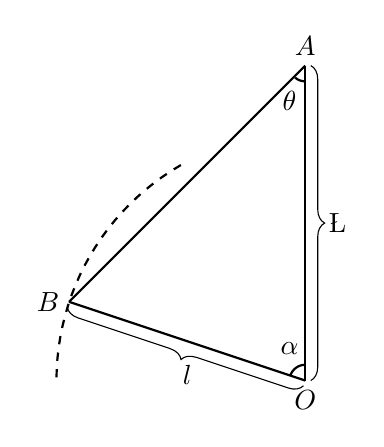
\begin{tikzpicture}[scale=1]
	
	% triangle
	\node[black, below] at (0,0) {$O$};
	\node[black, above] at(0,4) {$A$};
	\node[black, left] at(-3,1) {$B$};
	
	\draw[-, thick, black] (0,0) -- (0,4);
	\draw[-, thick, black] (0,4) -- (-3,1);
	\draw[-, thick, black] (-3,1) -- (0,0);
	
	% arc de cercle centré en O passant par B
	\draw [black,thick, dashed,domain=120:180] plot ({3.16*cos(\x)}, {3.16*sin(\x)}) ;
	
	% angles alpha, theta
	\draw [black,thick,domain=90:160] plot ({.2*cos(\x)}, {.2*sin(\x)});
	\node[below] at (-.2,.6) {$\alpha$};
	\draw [black,thick,domain=-90:-130] plot ({.2*cos(\x)}, {4+.2*sin(\x)});
	\node[below] at (-.2,3.8) {$\theta$};
	
	% length braces
	\draw [decorate,decoration={brace,amplitude=5pt,mirror, raise=2pt}]
(-3,1) -- (0,0) node[midway, below = 5pt]{$\l$};
	\draw [decorate,decoration={brace,amplitude=5pt,mirror, raise=2pt}]
(0,0) -- (0,4) node[midway, right = 5pt]{$\L$};
\end{tikzpicture}
\end{center}

\exe{}{
	Dessiner le projeté orthogonal $I$ de $B$ sur $(OA)$ qui définit la hauteur du triangle $OAB$ issue de $B$.
	On pose $h = BI$ cette hauteur.
}{exe:q1}{
	$I$ est placé sur $(OA)$ tel que $(BI)$ et $(OA)$ soient perpendiculaires.
	
%	\begin{center}
%	\begin{tikzpicture}[scale=1]
%		
%		% triangle
%		\node[black, below] at (0,0) {$O$};
%		\node[black, above] at(0,4) {$A$};
%		\node[black, left] at(-3,1) {$B$};
%		
%		\draw[-, thick, black] (0,0) -- (0,4);
%		\draw[-, thick, black] (0,4) -- (-3,1);
%		\draw[-, thick, black] (-3,1) -- (0,0);
%		
%		% arc de cercle centré en O passant par B
%		\draw [black,thick, dashed,domain=120:180] plot ({3.16*cos(\x)}, {3.16*sin(\x)}) ;
%		
%		% angles alpha, theta
%		\draw [black,thick,domain=90:160] plot ({.2*cos(\x)}, {.2*sin(\x)});
%		\node[below] at (-.2,.6) {$\alpha$};
%		\draw [black,thick,domain=-90:-130] plot ({.2*cos(\x)}, {4+.2*sin(\x)});
%		\node[below] at (-.2,3.8) {$\theta$};
%		
%		% length braces
%		\draw [decorate,decoration={brace,amplitude=5pt,mirror, raise=2pt}]
%	(-3,1) -- (0,0) node[midway, below = 5pt]{$\l$};
%		\draw [decorate,decoration={brace,amplitude=5pt,mirror, raise=2pt}]
%	(0,0) -- (0,4) node[midway, right = 5pt]{$\L$};
%	
%		% projeté orthogonal
%		\draw[-, RED_E, dashed] (-3,1) -- (0,1) node[midway, above]{$h$};
%		\node[RED_E, right] at(0,1) {$I$};
%	\end{tikzpicture}
%	\end{center}
}

\exe{}{
	Montrer que
		%\[ h = \l\sin(\alpha). \]
		$ h = \l\sin(\alpha) $
		et 
		$ OI = \l\cos(\alpha). $
}{exe:q2}{
	Dans le triangle $OBI$ rectangle en $I$, la trigonométrie nous donne
		\begin{align*}
			\sin(\alpha) = \dfrac{BI}{OB} = \dfrac{h}{\l} && \et && \cos(\alpha) = \dfrac{OI}{OB} = \dfrac{OI}{\l}.
		\end{align*}
	En multipliant par $\l$, on obtient bien $h = \l\sin(\alpha)$ et $OI = \l\cos(\alpha)$.
}

%\exe{}{
%	Montrer que la base $OI$ est donnée par
%		
%		%\[ OI = \l\cos(\alpha). \]
%}{exe:q3}{
%	Dans le triangle $OBI$ rectangle en $I$, la trigonométrique nous donne
%		\[ \cos(\alpha) = \dfrac{OI}{OB} = \dfrac{OI}{\l}. \]
%	En multipliant par $\l$, on obtient bien $OI = \l\cos(\alpha)$.
%}

\exe{}{
	Montrer que
		\[ \tan(\theta) = \dfrac{\l \sin(\alpha)}{\L - \l \cos(\alpha)}. \]
}{exe:q4}{
	Dans le triangle $ABI$ rectangle en $I$, la trigonométrie nous donne
		$ \tan(\theta) = \dfrac{BI}{AI}. $
	Or, d'après la question \ref{exe:q2},
		\begin{align*}
			BI = h = \l\sin(\alpha), && \et && AI = AO - OI = \L - \l\cos(\alpha).
		\end{align*}
	En conclusion,
		\[ \tan(\theta) = \dfrac{\l\sin(\alpha)}{\L - \l\cos(\alpha)}. \]
}

\exe{}{
	%En approximant à $10^{-4}$ , compléter les tableaux de valeurs de la fonction $f$ donnée algébriquement par
	Nous cherchons donc le maximum de la fonction $f$ suivante.
		\[ f(\alpha ) = \arctan\biggl(\dfrac{\l \sin(\alpha)}{\L - \l \cos(\alpha)}\biggr) \]
	Pour ceci, ouvrir l'activité Capytale (accès ENT) avec le code \textbf{9f11-10509009} et répondre aux questions suivantes.
	\begin{enumerate}
		\item
		Exécuter le code introductif et passer le premier test.
		\item
		Définir les variables $OA$ et $OB$ ainsi que la fonction $f$ puis passer le deuxième test.
		\item
		Tracer la courbe représentative de $f$ en parcourant l'intervalle $[0;90]$ en augmentant successivement le nombre d'antécédents.
		En déduire, approximativement, l'angle $\alpha$ permettant de maximiser $f(\alpha)$.
		\item
		%Calculer les coordonnées à $10^{-4}$ près du point d'abscisse $\alpha^\star = \arccos\bigl(\frac{\l}{\L}\bigr)$ appartenant $\C_f$ puis placer le point sur la courbe de la question précédente.
		Placer le point d'abscisse $\alpha^\star = \arccos\bigl(\frac{\l}{\L}\bigr)$ sur la courbe de la question précédente.
	\end{enumerate}
}{exe:q5}{
	\begin{center}
	\begin{tikzpicture}[>=stealth, scale=1]
		\begin{axis}[
			xmin=0,
			xmax=90, 
			ymin=0, 
			ymax=\ymaxplot,
			axis x line=middle,
			axis y line=middle,
			axis line style=-, 
			clip=false, 
			xtick distance = 10,
		]
			\addplot[BLUE_E, thick, domain=0:90, samples=100] {atan(\l*sin(x)/(\L - \l*cos(x)))}  node[right] {$\mathcal{C}_f$};
			
			\addplot[RED_E, very thick, mark=*, mark size = 1] (\xmax, \ymax) node[above] {$\color{RED_E} \bigl(\alpha^\star, f(\alpha^\star)\bigr)$};
%			\addplot[RED_E, very thick, mark=-, mark size = 1] (0,\hbeta) node[below] {$\color{RED_E} f(x^\star)$};
%			\draw[PURPLE, dashed, very thick] (axis cs:\xstar, 0) -- (axis cs:\xstar, \hbeta);
%			\draw[RED_E, dashed, very thick] (axis cs:0, \hbeta) -- (axis cs:\xstar, \hbeta);
		\end{axis}
	\end{tikzpicture}
	\end{center}
}

% VERY GOOD but i prefer to make them use Python right now
%
%	\begin{center}
%	\hspace{-1cm}
%	\begin{tabular}{|c|c|}\hline
%		$\alpha$ & $f(\alpha)$ \\ \hline
%		$\sampleI$ & \\ \hline
%		$\sampleII$ & \\ \hline
%		$\sampleIII$ & $\imageIII$\\ \hline
%		$\sampleIV$ & \\ \hline
%	\end{tabular}
%	\hfill
%	\begin{tabular}{|c|c|}\hline
%		$\alpha$ & $f(\alpha)$ \\ \hline
%		$\sampleV$ & \\ \hline
%		$\sampleVI$ & \\ \hline
%		$\sampleVII$ & \\ \hline
%		$\sampleVIII$ & $\imageVIII$ \\ \hline
%	\end{tabular}
%	\hfill
%	\begin{tabular}{|c|c|}\hline
%		$\alpha$ & $f(\alpha)$ \\ \hline
%		$\sampleIX$ & \imageIX \\ \hline
%		$\sampleX$ & \\ \hline
%		$\sampleXI$ & \\ \hline
%		$\sampleXII$ & \\ \hline
%	\end{tabular}
%	\hfill
%	\begin{tabular}{|c|c|}\hline
%		$\alpha$ & $f(\alpha)$ \\ \hline
%		$\sampleXIII$ & \\ \hline
%		$\sampleXIV$ & \\ \hline
%		$\sampleXV$ & $\imageXV$ \\ \hline
%		$\sampleXVI$ & \\ \hline
%	\end{tabular}
%	\hfill
%	\begin{tabular}{|c|c|}\hline
%		$\alpha$ & $f(\alpha)$ \\ \hline
%		$\sampleXVII$ & $\imageXVII$ \\ \hline
%		$\sampleXVIII$ & \\ \hline
%		$\sampleXIX$ & \\ \hline
%		$\sampleXX$ & \\ \hline
%	\end{tabular}
%	\end{center}

%\exe{
%	Tracer $\C_f$ dans un repère de domaine $[0; 90]$ et estimer l'angle $\alpha^\star \in [0;90]$ pour lequel $f(\alpha^\star)$ est maximal.
%}{}

\exe{, difficulty=1}{
	Nous souhaitons nous convaincre que le point d'abscisse $\alpha^\star$ placé à l'exercice \ref{exe:q5} est situé au pic de la fonction, et donc que $f(\alpha^\star)$ est le maximum de $f$ sur $[0;90]$.
	
	\begin{enumerate}
		\item 
		Quelle inégalité doit vérifier $\alpha^\star$ ?
		Est-il possible de la vérifier algorithmiquement ?
		\item
		Écrire un algorithme à la fin de l'activité Capytale permettant de parcourir le domaine avec pas $10^{-4}$ et de vérifier cette inégalité.
		Combien de valeurs l'algorithme a-t-il parcouru ?
	\end{enumerate}
}{exe:q6}{
	Il s'agit de vérifier que
		\[ f(\alpha) \leq f(\alpha^\star) \]
	pour tout $\alpha \in [0;90]$.
	
	Attention au domaine $[0;90]$ dans lequel $\alpha$ vit ici : l'angle peut prendre une infinité de valeurs différentes.
	Par conséquent, un algorithme par balayage ne permet pas de vérifier cette inégalité, car un tel algorithme doit parcourir un nombre fini d'antécédents $\alpha$ pour qu'il termine.
	Notons cependant qu'un algorithme plus sophistiqué ou dans un langage plus adapté pourrait démontrer notre inégalité :
	les assistants de preuve \emph{Lean} et \emph{Rocq} ont été créés dans le but faire vérifier par la machine les preuves mathématiques difficiles.
	
	Pour se convaincre du caractère optimal de notre solution (sans le démontrer, donc !), nous pouvons alors parcourir l'intervalle avec un pas très petit ($10^{-4}$ par exemple) et vérifier l'inégalité pour chaque antécédent $\alpha$.
	
	\texttt{\\
	for x in np.arange(0,90,.0001): \\
	\null\qquad if f(x) > f(xetoile):\\
		\null\qquad\qquad print("ATTENTION : ", x)
	}
	
	Ceci prend un certain temps car il y a $90\times10^4 = 900~000$ antécédents à tester.
	Au final, rien n'est imprimé par l'algorithme : il n'y a aucun \texttt{x} tel que \texttt{f(x) > f(xetoile)}.
	
}


%%%%%%%%%%%%%%%%%%%
%%%%%%%%%%%%%%%%%%%
%%%%%%%%%%%%%%%%%%%

\newpage
\fancyhead[C]{\textbf{Solutions -- {\seed} -- Trigonométrie}}
\fakesection{Solution \seed}
\shipoutAnswer

\end{document}

